\chapter{Placa de Circuito Impreso (PCI)}
\section{Introducción}
La placa de circuito impreso es un componente electrónico de tipo electromecánico que permite el ensamblado del resto de los componentes electrónicos necesarios para asegurar la funcionalidad del sistema electrónico. Facilita el soporte físico y el interconexionado de los componentes y permite la integración dentro del resto del conjunto.

Criterios de clasificación de las PCIs:
\begin{itemize}
    \item Materiales utilizados en la construcción de la PCI. Orgánicos (resinas fenólicas, pasta de papel, fibra de vidrio) ó compuestos no orgánicos (cerámicos, aluminio, etc.)
    \item Tipo de conductor. Pistas conductoras de cobre base por etching químico (trama gráfica), deposición de capa gruesa ó cableado directo (wire-bonding)
    \item Rigidez mecánica de la PCI. Rígidas, flexibles ó mixtas.
    \item Método de formación de las pistas conductoras. Técnicas sustractivas del cobre: eliminando parte del cobre sobrante (etching químico), ó técnicas aditivas: se añade cobre, pastas conductoras ó cable conductor.
    \item Número de capas conductoras. Monocapa, bicapa ó multicapa.
    \item Uso de vías de interconexión entre capas (PTH).
\end{itemize}

\subsection{Materiales utilizados en la cosntrucción de la PCI}
\subsubsection{Orgánicos}
La PCI de papel fenócilo CEM tiene un color ocre (mostaza), es de bajo coste y se utiliza en aplicaciones no profesionales. Son sólo placas monocapas con baja estabilidad térmica (se deforman fácilmente con la temperatura), no permiten alta densidad de pistas ni de pads de soldadura, no son adecuadas para montajes SMT. Se fabrican en plantas diferentes de las de fibra de vidrio por los residuos que generan.

La PCI de fibra de vidrio FR4 es la más usads, tiene un color verde ó azul. Incorporan susbstancia retardante a la llama (FR). Tienen un mayor coste y se utilizan en aplicaciones profesionales. Son muy estables térmicamnete, permiten soluciones bicapa y multicapa (hasta 48), alta densidad de pistas y pads de soldadura, admiten thorugh-hole y SMT, y tienen acabados superficiales en Sn y Au.

\subsubsection{No orgánicos}

La PCI de aluminio tiene un elevado coste, altas prestaciones térmicas y se utiliza para aplicaciones profesionales (automoción, defensa y aeroespacial), son principalmente monocapa, aunque pueden ser bicapa depositando una capa gruesa de aislante. Son muy utilizados en módulos multichip, convertidores DC/DC por su facilidad de disipación de calor.

La PCI de substrato cerámico tiene un elevado coste, altas presatciones térmicas y se utiliza para aplicaciones profesionales (automoción, defensa y aeroespacial), son principalmente monocapa, aunque pueden ser bicapa depositando una capa gruesa de aislante. Se usan en circuitos híbridos.

\subsection{Tipo de conductor}
\subsubsection{Etching de cobre}
\begin{enumerate}
    \item Se parte de una lámina aislante, cubierta con una lámina uniforme de CU de $35 \mu m$ de espesor.
    \item Se retira el cobre sobrante por ataque químico (etching) hasta dejar las pistas y los pads.
\end{enumerate}
 
\subsubsection{Deposición de capa gruesa}
\begin{enumerate}
    \item Se parte de un substato aislante rígido (cerámico=
    \item Se deposita pasta conductora para conformar las pistas y pads de soldadura por técnicas serigráficas.
    \item Se procede a curado en horno a alta temperatura para retirar el disolvente de la pasta conductora.
    \item Una vez curado, las pistas quedan solidificadas.
    \item Se pueden añadir pistas aislantes.
    \item Se pueden incorporar resistencias por deposición de capa gruesa.
\end{enumerate}

\subsubsection{Wire bonding}
Es una técnica de interconexionado por cableado con hilo fino. Aplica la técnica de termocompresión mediante aguja. Requiere un substrato rígido (FR, Aluminio, Cerámico). Es la base de la técnica COB (Chip On Board). Permite altas densidades de conexionado, reduce la superficie de la PCI ya que el CI no lleva encapsulado, requiere de un acabado final de recubrimiento de resina epoxy para proteger al CI.

\subsection{Rigidez mecánica de la PCI}
\subsubsection{Rigidas}
No se deforman. Son de papel fenólico (CEM), fibra de vidrio (FR), aluminio o cerámica.

\subsubsection{Flezibles}
Se pueden curvar. Son de substrato de acetato flexible.

\subsubsection{Mixtas}
Se forman combinando en la PCI una parte rígida y otra flexible. Se utilizan para interconexionar elementos que pueden girar (pantallas, teclados, etc...).

\subsection{Número de capas}
\subsubsection{Monocapas}
Llevan componentes en una sola cara (top layer) normalmente through-hole. Las pistas y pads se obtienen por serigrafía y posterior ataque químico del Cu sobrante. Se utiliza en aplicaciones de bajo coste y circuitos simples con pocos componentes.

\subsubsection{Bicapas}
Llevan 2 capas conductoras (top y bottom) y el material aislante (FR4). El circuito puede llevar componentes en ambas caras de la placa. Se pueden montar tanto componentes through-hole como SMT. Permiten altas densidades de componentes y de pistas. Se utiliza el FR4 por su estabilidad térmica.

\subsubsection{Multicapas}
Sólo llevan componentes en las capas externas (top y bottom). Además de las capas externas, llevan varias internas formando un sándwich de capas conductoras y aislantes. Se fabrican laminando, placas de cara simple ya separadas (transferencia de imagen) con FR4 como aislante. La interconexión entre las diferentes capas se realiza a través de taladros específicos de paso denominados vías.

\subsection{Tipos de taladros}

\subsubsection{Placas Monocapa}

\begin{figure}[H]
    \centering
    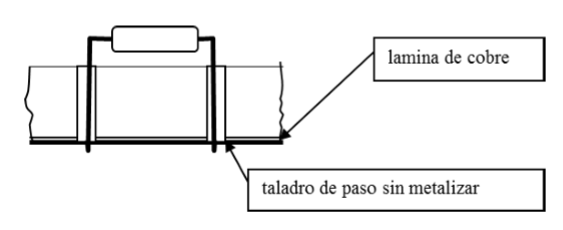
\includegraphics[width=0.5\linewidth]{Imagenes/PCI - Taladros Monocapa.png}
\end{figure}

Llevan taladros de paso SIN metalizar, para permitir el montaje de componentes through-hole. El componente se monta por la cara top y se suelda al pad de soldadura en la cara bottom.

\subsubsection{Placas Bicapa}

\begin{figure}[H]
    \centering
    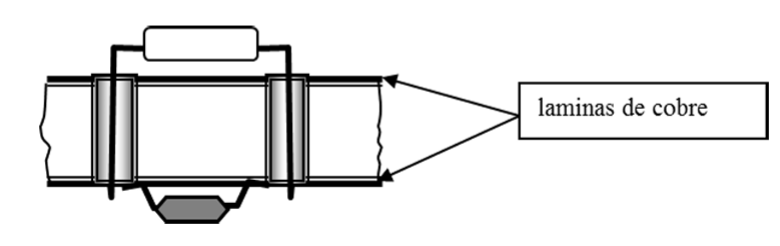
\includegraphics[width=0.5\linewidth]{Imagenes/PCI - Taladros Bicapa.png}
\end{figure}

Llevan taladros metalizados (plated through holes PTH). Los taladros sse metalizan en su interior, una vez hechos. Al pasar la PCI por la ola de estaño, éste entra y sube por el taladro, por capilaridad y asegura el contacto y la sujeción mecánica del componente electrónico.

\subsubsection{Placas Multicapa}

\begin{figure}[H]
    \centering
    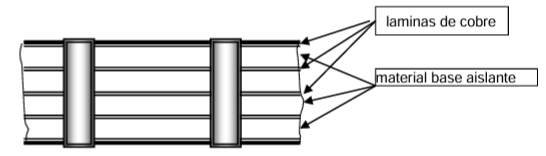
\includegraphics[width=0.5\linewidth]{Imagenes/PCI - Placas Multicapa.png}
\end{figure}

Llevan varios tipos de taladros: PTH para montaje de los componentes through-hole, y de paso (via holes) para el interconexionado interno entre capas. Todos son metalizados.

\section{Fases del proceso de fabricación}

\begin{enumerate}
    \item Fabricación del substrato
    \item Procesos de serigrafía o fotograbado
    \item Construcción de las vías: taladrado
    \item Cobreado catalítico
    \item Cobreado electrolítico
    \item Ataque químico de pistas externas
    \item Placas multicapa: apilamiento y prensado de capas
    \item Mecanizado de contornos
    \item Protección contra ataque químico mediambiental. Acabado superficial (Sn, Au)
    \item Recubrimiento con máscaras antisoldadura (solder mask)
    \item Test de la PCI (continuidad de pistas, aislamiento...)
\end{enumerate}

\subsection{Fabricación del substrato}
\subsubsection{Proceso de laminado}
Consiste en unir varias capas de material base para ser tratadas y curadas. Posteriormente se procede a depositar sobre las mismas una fina película de cobre, cuyo espesor final depende del número de láminas depositadas. Esta deposición de cobre se puede hacer sobre una cara o sobre las dos.

\subsubsection{Prensado}
El estratificado se somete a un proceso de prensado a alta temperatura mediante una prensa hidráulica. Posteriormente se enfría hasta alcanzar la temperatura ambiente. Se obtienen finas planchas de gran tamaño de material aislante cubierto por 1 ó 2 capas de cobre de 35um de espesor.

\subsubsection{Calidad y fiabilidad}
Requisitos cualitativos que han de cumplir los laminados:
\begin{itemize}
    \item Superficie de cobre: ausencia de salientes.
    \item Fuerza de delaminación: permite comprobar la adherencia del cobre al substrato.
    \item Combado y revirado: determina el grado de deformación de la placa por unidad de superficie.
    \item Resistencia a la soldadura: se comprueba la resistencia del substrato y la adherencia de la lámina de cobre a un proceso de soldadura. Se comprueba la ausencia de levantamiento, delaminación, y corrugamiento.
    \item Resistencia de aislameinto: especifica la resistencia entre dos conductores de una misma lámina.
    \item Rigidez dieléctrica: indica el grado de resistencia que puede ofrecer el substrato a una descarga eléctrica disruptiva producida por un ensayo eléctrico.
\end{itemize}

\subsection{Mecanizado de la PCI}
\subsubsection{Cortado de la placa}
Se cortan por cizalla para obtener las planchas con las dimensiones adecuadas al proceso de fabricación. En algunos casos, también se utilizan sierras de corte circulares.

\subsubsection{Enrutado ó fresado}
Permite obtener el contorno de la PCI a las dimensiones y geometrías en función del diseño mecánico, extraer material, etc. La máquina consta de un pequeño cilindro de carburo que gira a una velocidad de 12000-24000 rpm, de forma que puede cortar el grosor de la placa de circuito impreso normalmente de control numérico CNC. Se puede guiar libremente sobre la placa, pudiendo dibujar cualquier forma. También permite hacer taladros de gran diámetro para sujeción mecánica.

\subsubsection{Taladrado}
Es uno de los procesos más costosos, cuidadoso y que requiere mayor precisión. Se realiza para obtener los taladrros y vías de la PCI del diámetro adecuado. Para asegurar la calidad, las brocas son de tungsteno con distintas geometrías en función del material a taladrar y su uso está limitado a un número limitado de operaciones. Las mejores brocas producen una temperatura de taladrado menor, una superficie de corte más abrupta, y no generan rebabas, etc.

La placa o substrato será aprisionada durante el taladrado entre una placaa de material de entrada y una placa de salida. La placa de material de entrada se usa para prevenir daños en la superficie superior del circuito impreso. La placa de salida (backup) se sitúa bajo el circuito impreso y será atravesada por la broza para prevenir que se pueda fracturar la parte inferior de la placa. Como placa de entrada se usan distintos materiales: aluminio sólido, pasta de papel, o pastas basadas en resina en proporción de 60\% de papel y 40\% de resina. Para la placa de salida se usan láminas de pasta basada en resina con 40\% de papel y 60\% de resina, o láminas duras prensadas de fibra vegetal con resina y aceites.

\subsection{Metalización de taladros}
Este proceso permite metalizar el interior de los taladros en PCIs bicapa y multicapa. Previamente se procede a la limpieza del interior de las vías (rebabas de material conductor, restos de material aislante) para evitar problemas de conexionado en PCIs multicapa. Se realiza normalmente con productos químicos. A posteriori, se procede a la metalización catalítica (química) del interior con Cu y posteriormente con Pd y Sn.

\subsubsection{Metalización electrolítica del Cu de la PCI}
Permite recrear la película de Cu de la PCI (inicialmente de 35 um) a un espesor mayor. Se realiza por procedimientos electrolíticos.

\subsection{Obtención de pistas}
Proceso mediante el cual se elaboran las pistas, pads de soldadura, contactos, etc...de la PCI. Estos elementos permiten la interconexión de los componentes (para asegurar la funcionalidad del circuito), así como su sujeción mecánica a través de la soldadura. La transferencia de la imagen de las pistas se hace por fotograbado (técnica fotolitográfica).

\subsubsection{Fotograbado por película seca}
\begin{enumerate}
    \item Depegar la película protectora de celofán (poliolefina) de la lámina de material protector a depositar.
    \item Queda así al descubierto la película fotosensible, negativa o positivia, que se adhiere a la capa superficial de cobre.
    \item La película seca fotosensible queda protegida por una lámina delgada de poliester, que evita daños a la película fotosensible y al cliché de pistas.
    \item Aplicar el cliché sobre la película de poliéster.
    \item Irradiar verticalmente con la fuente luminosa a la que es sensible la capa seca.
    \item Para transferir las pistas del cliché, la capa fotosensible cambia sus características de solubilidad en el revelador en aquellas zonas que han sido irradiadas, es decir, las zonas transparentes del cliché.
    \item Despegar la capa protectora de poliéster. Queda al descubierto la película seca fotosensible irradiada en el paso anterior.
    \item Sumergir en el baño de revelado según sea la película fotosensible positiva ó negativa.
    \item En el proceso de revelado se elimina la fotorresina irradiada ó la no irradiada-.
    \item Quedan al descubierto las zonas de cobre cuya cubierta de película seca ha sido disuelta en el proceso de revelado.
\end{enumerate}

\subsubsection{Ataque químico}
Es un proceso substractivo que elimina el cobre no deseado de los substratos, para de esta forma crear el conjunto de pistas conductoras y pads. Se pueden obtener pistas de anchuras muy finas, entre 0,1 y 0,15 mm hasta varios mm para pistas de alimentación y masa. 
\begin{enumerate}
    \item Una vez depositada la capa resistente al ataque químico sobre las zonas a conservar metalizadas de la superficie del substrato, la placa se introduce en un baño con la solución corrosiva.
    \item Esta solución elimina todo el cobre de la superficie de la placa, excepto en aquellas áreas que se encuentran protegidas por el material no atacable.
    \item Después de que todo el cobre no necesario es eliminado, la placa pasa a una estación de limpieza, donde se lava la solución corrosiva residual, y el material no atacable que protegió inicialmente las pistas (restos de la película fotosensible polimerizada).
    \item Mientras la placa está en contacto con la solución corrosiva, el ataque se realiza en todas las superficies que están en contacto con la solución (ataque isotrópico).
    \item También se produce un ataque bajo el material resistivo, ya que la solución penetrará bajo éste.
    \item Este ataque es el origen del fenómeno del undercutting, y el efecto del ataque lateral de la pista protegida.
    \item La relación entre la profundidad lateral (Y) y la vertical (X) se denomina factor de ataque.
    \item Eliminación de la película seca que recubre al cobre no atacado con producto disolvente.
    \item Limpieza para eliminar restos de los productos utilizados en pasos anteriores y dejar la superficie de cobre de las pistas sin restos de óxidos o sales.
    \item Almacenamiento en atmósfera seca e inerte que no produzca reacción química en la superficie de la PCI.
\end{enumerate}

\subsection{Mecanizado de contornos}
\subsubsection{Fresado}
Operación de fresado CNC. Permite conformar el contorno de la PCI. Eliminar material FR4 sobrante. Realizar taladros de gran tamaño para sujeción mecánica.

\subsubsection{Por broca}
La operación es similar al proceso de taladrado por broca. Se procede a dar el último contorno, y las eliminaciones de materia prima para facilitar el despanelizado de placas. Se aplica mayormente en placas en las que la forma final no es totalmente simétrica, y tiene algunas curvaturas.

\subsubsection{V Scoring}
Este método consiste en realizar un corte en la PCI de tal manera a debilitar su espesor. El V-SCORING se realiza con una sierra circular que produce una mella en forma de V con un espesor determinado y calibrado. Facilita la separación de las PCIs del panel (despanelizado).

\subsection{Acabado de pistas, contactos y taladros}
El Cu altamente sensible a corrosión y oxidación, lo cual dificulta la soldadura de componentes. Para evitar este problema, se procede a realizar un acabado del cobre expuesto. Este acabado puede ser de 3 tipos, según la aplicación de la PCI, requisitos de fiabilidad, tiempo de almacenamiento:
\begin{itemize}
    \item Acabado estañado (Hol Air Leveling - HAL)
    \item Acabado en Au químico
    \item Acabado en Au electrolítico
\end{itemize}

\subsubsection{Acabado HAL}
Consiste en depositar sobre las zonas expuestas de cobre, una película de una aleación de Sn. Se aplica la técnica de HAL: consiste en sumergir la placa totalmente en un crisol con la aleación de Sn fundida y sacarla gradualmente. Al salir, se hace pasar por unas cuchillas de aire caliente, cuya misión es la de refundir el Sn sobrante, de manera a retirar el estaño superfluo que haya podido quedar sobre los contactos, dentro de los taladros, y sobre algunas pistas.

\subsubsection{Acabado en Au químico}
La deposición del Au químico se realiza por procedimientos químicos. Permite crear una capa uniforme de espesores de unas 75 um, sobre toda la PCI. Se aplica para obtener un elevado grado de inmunidad contra corrosión y oxidación de las partes conductoras expuestas a intemperie. Aumenta la fiabilidad de la PCI. Requisito importante para montar componentes de montaje superficial (SMT) y requisito imprescindible para el montaje COP por wirebonding.

\subsubsection{Acabado en Au electrolítico}
El Au se deposita por procedimiento electrolítico. Permite obtener mayores espesores que el procedimiento químico. Tan sólo se puede aplicar a los extremos de la PCI, por lo que se aplica principalmente en el dorado de contactos para placas encartables. Aumenta la dureza de los contactos lo que permite aumentar el número de operaciones de conexión/desconexión de la PCI. Inmuniza contra corrosiones.

\subsection{Mascarilla antisoldante}
Se deposita sobre la PCI, y constituye una de las útlimas fases del proceso de fabircación. Se utiliza para proteger a las pistas conductoras contra corrosión y arañazos, y evitar cortocircuitos en el proceso de3 soldadura de componentes por exceso de Sn en la ola de soldar (Through-hole) ó en el horno de refusión (SMT). Es la causa del aspecto verdoso/azulado de la PCI.

\begin{enumerate}
    \item Se aplica tinta (mascarilla antisoldante) a toda la placa.
    \item Se procede al insolado con rayos UV con un cliché de forma similar a como se hizo en film seco, para al revelar y dejar sin tinta los taladors donde se insertarán (through-hole) o soldarán (smd) los componentes.
    \item Se somete a curado para conseguir la polimerización de la máscara. La máscara queda endurecida y adherida a la PCI.
\end{enumerate}

\subsection{Verificación}
Una vez terminada de fabricar la PCI, se ha de proceder a realizar varias verificaciones, antes de ser enviada al cliente final para que proceda al ensamblado con los componentes.

\subsubsection{Inspección}
Al acabar el proceso de fabricación, se realiza una inspección visual de varios puntos que puede comprender:
\begin{itemize}
    \item Ausencia de marzas de arañazo
    \item Falta de soldermask en alguna zona
    \item Serigrafía correcta
    \item Ausencia de daño aparente en la PCI
    \item Apariencia de los acabados (Sn/Pb, Au químico, Au electroliticio)
    \item Código de la PCI versión y marca de lote de fabricación son correctos y coinciden con los solicitados
    \item Dimensiones de la PCI y del panel
    \item Diámetro de taladros
\end{itemize}

Se puede realizar al 100\% de la producción o por muestreo (\% reducido de la producción). En el caso de hacerse por muestreo, y evidenciarse algún defecto, se procederá inmediatamente a inspeccionar toda la producción, para evaluar el impacto y proceder inmediatamente a reponer el material rechazado. Los criterios aplicables han de ser acordados con el cliente final.

\subsubsection{Test eléctrico}
Permite comprobar la funcionalidad eléctrica del circuito. La comprobación se realiza utilizando un equipo de test formado por:
\begin{itemize}
    \item Un ordenador con el SW de verificación que se encarga de aplicar la señal, y verificar el resultado, identificando aquellos puntos defectuosos.
    \item Una cama de pinchos, los cuales se sitúan en los puntos de test previstos al efecto en la PCI (test points). Estos pinchos en contacto con los puntos de prueba permiten aplicar la señal de verificación y leer en el otro extremo el resultado obtenido.
\end{itemize}

\textbf{Cortocircuitos:} Se producen al quedar dos elementos conductores adyacentes unidos por un residuo de Cu, bola de Sn, etc.

\textbf{Circuitos abiertos ó pistas cortadas:} Este defecto se da ucando una pista está interrumpida. Se puede producir por exceso de ataque químico, por fallo en el cliché, etc.

\textbf{Pistas debilitadas:} se produce por falta de material conductor en alguna pista, o algún pad. No produce defecto eléctrico a priori, pero puede dar lugar a problemas a corto plazo. Se puede detectar con el sistema de AOI (Inspección automática óptica).

\subsubsection{Auditoría final de calidad}
La realiza el Departamento de Calidad sometiendo muestras a un ensayo más exhaustivo, utilizando para ello, probetas metalográficas a partir de las cuales puede determinar la calidad de los acabados, recubrimientos interiores, etc. Se comprueba la ausencia de los defectos más importantes que se puedan presentar.

\section{Diseño y documentación de las PCIs}
Las PCIs son componentes electrónicso diseñados específicamente para el dispositivo en el que se va a montar. No existen como tal en el mercado. Se fabrican en instalaciones industriales especializadas, con herramientas automatizada, basadas la mayoría en CNC. El diseñador de la PCI ha de elaborar toda la documentación, la cual hab´ra de ser remitida al fabricante, para que inicie el proceso de fabricación. Esta documentación ha de elaborarse en base a los requisitos de CAD/CAM del fabricante. Se utilizan formatos estándar adoptados tanto por diseñadores como por fabricantes.

Documentos a elaborar:
\begin{itemize}
    \item Ficheros GERBER (proporcionados por el SW de diseño de la PCI)
    \item Planos de pistas
    \item Planos de taladros
    \item Planos de mecanizado
    \item Ruedas de apertura (incluida en los ficheros GERBER), que incluyen todos los tipos de taladros, coordenadas en la PCI, diámetro, acabado, función, etc...
    \item Solder mask cara top
    \item Solder mask cara bottom
    \item Soldering paste top
    \item Soldering paste bottom
    \item Silk screen (serigrafía)
\end{itemize}

\subsection{Ficheros GERBER}
Los ficheros GERBER son el estándar más utilizado como formato de elaboración de documentación de diseño, compatible con recursos CAD/CAM tanto por diseñadores como por fabricantes de PCIs. Facilita la transferencia de datos entre diseñado y fabricante, mediante métodos electrónicos. Asegura que el fabricante dispone de la documentación correcta y actualizada en versión. Permite al fabricante generar su propia documentación para la fabricación. Tan solo tiene que transferir y adaptas los ficheros recibidos. Los ficheros GERBER los genera el SW de diseño de la PCI, como exportación de documentos.

\subsection{Plano de taladrado}
\begin{itemize}
    \item Coordenadas X-Y respecto de un punto de referencia fiducial
    \item Número de taladros
    \item Diámetro de cada uno
    \item Tolerancias en diámetro y posición
    \item Tipo (metalizado, no metalizado)
\end{itemize}

\subsection{Plano de mecanizado}
\begin{itemize}
    \item Dimensiones, grosor PCI, tolerancias
    \item Panelizado
    \item Mecanizado final (fresado, V scoring, etc.)
    \item Acabado superficial parte conductora (Sn, Au, etc.)
    \item Acabados final (solder mask)
\end{itemize}

\subsection{Especificaciones de Calidad y Fiabilidad}
Se especifican todos los requisitos de la Calidad y la Fiabilidad que han de cumplir la PCI y el fabricante ha de asegurar y de certificar. Las especificaciones han de hacer referencia a los distintos cristerios de inspección para los distintos tipos de parámetros:
\begin{itemize}
    \item Acabado. Ausencia de señales de daño físico.
    \item Dimensiones de la PCI.
    \item Diámetros de taladros
    \item Anchura y grosor de pistas
    \item Nivel de Calidad (máximo número de unidades defectuosas admisibles por lote)
    \item Requisitos de inspección óptica
    \item Requisitos de inspección eléctrica
    \item Ensayos mecánicos (soldadura, desprendimiento de pistas, etc...)
\end{itemize}

\subsection{Certificado del fabricante}
En base a los requisitos establecidos por el diseñador, el fabricante ha de remitir con cada envío de lotes de PCIs, un certificado en el que haga constar todos los datos y resultados del proceso de inspección y de aseguramiento de la Calidad y de la Fiabilidad del lote remitido. Este certificado, una vez recibido por el diseñador, éste pueda confirmar que efectiva, ente se cumplen. En caso de detectar fallos, defectos ó incumplimientos, este recurso le permite al diseñador argumentar contra el fabricante.